\section{Preventivo}

	Per facilitare la lettura del documento e delle tabelle sono stati adottati delle sigle per indicare i vari ruoli in modo più sintetico:
	\begin{itemize}
		\item \textbf{An:} analista;
		\item \textbf{Amm:} amministratore;
		\item \textbf{Pr:} programmatore;
		\item \textbf{Pt:} progettista;
		\item \textbf{Re:} responsabile;
		\item \textbf{Ve:} verificatore.
	\end{itemize}

%
%
% Individuazione degli strumenti e analisi dei requisiti
%
%
\subsection{Individuazione degli strumenti e analisi dei requisiti}

\subsubsection{Prospetto orario}

Nella fase di autoformazione e individuazione degli strumenti ogni componente rivestirà i seguenti ruoli:
\begin{longtable}{|c|c|c|c|c|c|c|c|}
	\hline
	\rowcolor[HTML]{F9CB9C} 
	\textbf{Nominativo} & \textbf{An} & \textbf{Amm} & \textbf{Pr} & \textbf{Pt} & \textbf{Re} & \textbf{Ve} & \textbf{Ore totali} \\
	\hline
	Calcagno Riccardo & 
	- & 
	5 & 
	- & 
	- & 
	0 & 
	5 & 
	20 \\
	\hline
	Michieletto Giovanni & 
	10 &
	4 & 
	- & 
	- & 
	- & 
	6 & 
	20 \\
	\hline
	Sartor Samuele & 
	8 & 
	4 & 
	- & 
	- & 
	- & 
	8 & 
	20 \\
	\hline
	Schiavon Vittorio & 
	7 & 
	- & 
	- & 
	5 & 
	- & 
	8 & 
	20 \\
	\hline
	Sinigaglia Alberto & 
	15 & 
	- & 
	- & 
	- & 
	- & 
	5 & 
	20 \\
	\hline
	Tesser Marco & 
	10 & 
	- & 
	- & 
	6 & 
	- & 
	4 & 
	20 \\
	\hline	
	Zago Alice & 
	6 & 
	8 & 
	- & 
	- & 
	- & 
	6 & 
	20 \\
	\hline	
	\rowcolor[HTML]{F9CB9C} 
	\textbf{Ore totali ruolo} & \textbf{56} & \textbf{21} & \textbf{-} & \textbf{11} & \textbf{10} & \textbf{42} & \textbf{140} \\
	\hline
	\caption{Prospetto orario individuazione degli strumenti e analisi dei requisiti.}
	\label{fig: Prospetto orario individuazione degli strumenti e analisi dei requisiti.}
\end{longtable}

I dati ottenuti si possono riassumere nel seguente istogramma:
\begin{figure}[H]
	\centering
	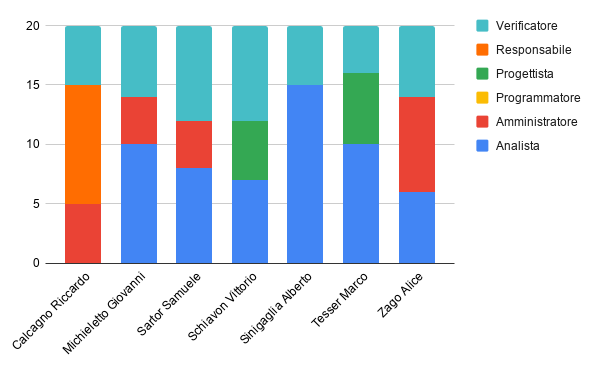
\includegraphics[width=0.8\linewidth]{./res/images/OreStrumentiRequisiti.png}
	\caption{Istogramma ore individuazione degli strumenti e analisi dei requisiti.}
	\label{fig: Istogramma ore individuazione degli strumenti e analisi dei requisiti.}
\end{figure}

\subsubsection{Prospetto economico}

In questa fase il costo per ogni ruolo è il seguente:
\begin{longtable}{|c|c|c|}
	\hline
	\rowcolor[HTML]{F9CB9C} 
	\textbf{Ruolo} & \textbf{Ore} & \textbf{Costo} \\
	\hline
	Analista & 
	56 & 
	1400 \\
	\hline
	Amministratore & 
	21 & 
	420 \\
	\hline
	Programmatore & 
	- & 
	- \\
	\hline
	Progettista & 
	11 & 
	242 \\
	\hline
	Responsabile & 
	10 & 
	300 \\
	\hline
	Verificatore & 
	42 & 
	630 \\
	\hline
	\rowcolor[HTML]{F9CB9C} 
	\textbf{Totale} & \textbf{140} & \textbf{2992} \\
	\hline
	\caption{Costi individuazione degli strumenti e analisi dei requisiti.}
	\label{fig: Costi individuazione degli strumenti e analisi dei requisiti.}
\end{longtable}

I dati ottenuti si possono riassumere nel seguente diagramma circolare:
\begin{figure}[H]
	\centering
	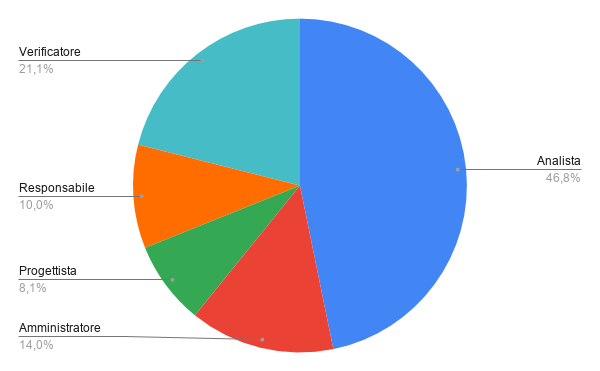
\includegraphics[width=0.6\linewidth]{./res/images/CostiStrumentiRequisiti.png}
	\caption{Diagramma circolare costi individuazione degli strumenti e analisi dei requisiti.}
	\label{fig: Diagramma circolare costi individuazione degli strumenti e analisi dei requisiti.}
\end{figure}

		

%
%
% Fase di analisi di dettaglio
%
%
\subsection{Fase di analisi di dettaglio}

\subsubsection{Prospetto orario}

Nella fase di Analisi di dettaglio ogni componente rivestirà i seguenti ruoli:
\begin{longtable}{|c|c|c|c|c|c|c|c|}
	\hline
	\rowcolor[HTML]{F9CB9C} 
	\textbf{Nominativo} & \textbf{An} & \textbf{Amm} & \textbf{Pr} & \textbf{Pt} & \textbf{Re} & \textbf{Ve} & \textbf{Ore totali} \\
	\hline
	Calcagno Riccardo & 
	6 &
	- &
	- &
	- &
	- &
	10 &
	16 \\
	\hline
	Michieletto Giovanni &
	6 &
	4 &
	- &
	- &
	- &
	6 &
	16 \\
	\hline
	Sartor Samuele & 
	2 &
	6 &
	- &
	- &
	- &
	8 &
	16 \\
	\hline
	Schiavon Vittorio & 
	8 &
	- &
	- &
	- &
	- &
	8 &
	16 \\
	\hline
	Sinigaglia Alberto & 
	- &
	- &
	- &
	- &
	6 &
	10 &
	16 \\
	\hline
	Tesser Marco & 
	10 &
	6 &
	- &
	- &
	- &
	- &
	16 \\
	\hline	
	Zago Alice & 
	6 &
	- &
	- &
	- &
	- &
	10 &
	16 \\
	\hline	
	\rowcolor[HTML]{F9CB9C} 
	\textbf{Ore totali ruolo} & \textbf{38} & \textbf{16} & \textbf{-} & \textbf{-} & \textbf{6} & \textbf{52} & \textbf{112} \\
	\hline
	\caption{Prospetto orario analisi di dettaglio.}
	\label{fig: Prospetto orario analisi di dettaglio.}
\end{longtable}

I dati ottenuti si possono riassumere nel seguente istogramma:
\begin{figure}[H]
	\centering
	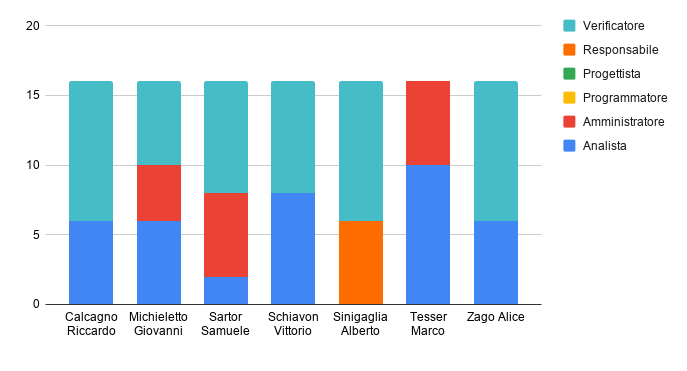
\includegraphics[width=0.8\linewidth]{./res/images/OreAnalisiDettaglio.png}
	\caption{Istogramma ore analisi di dettaglio.}
	\label{fig: Istogramma ore analisi di dettaglio.}
\end{figure}

\subsubsection{Prospetto economico}

In questa fase il costo per ogni ruolo è il seguente:
\begin{longtable}{|c|c|c|}
	\hline
	\rowcolor[HTML]{F9CB9C} 
	\textbf{Ruolo} & \textbf{Ore} & \textbf{Costo} \\
	\hline
	Analista &
	38 &
	950 \\
	\hline
	Amministratore &
	16 &
	320 \\
	\hline
	Programmatore &
	- &
	- \\
	\hline
	Progettista &
	- &
	- \\
	\hline
	Responsabile  &
	6 &
	180 \\
	\hline
	Verificatore &
	52 &
	780 \\
	\hline
	\rowcolor[HTML]{F9CB9C} 
	\textbf{Totale} & \textbf{112} & \textbf{2230} \\
	\hline
	\caption{Costi analisi di dettaglio.}
	\label{fig: Costi analisi di dettaglio.}
\end{longtable}

I dati ottenuti si possono riassumere nel seguente diagramma circolare:
\begin{figure}[H]
	\centering
	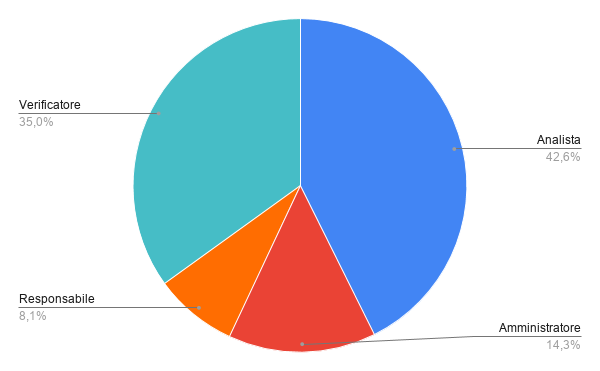
\includegraphics[width=0.6\linewidth]{./res/images/CostiAnalisiDettaglio.png}
	\caption{Diagramma circolare costi analisi di dettaglio.}
	\label{fig: Diagramma circolare costi analisi di dettaglio.}
\end{figure}

			

%
%
% Fase di progettazione architetturale
%
%
\subsection{Fase di progettazione architetturale}

\subsubsection{Prospetto orario}

Nella fase di progettazione architetturale ogni componente rivestirà i seguenti ruoli:
\begin{longtable}{|c|c|c|c|c|c|c|c|}
	\hline
	\rowcolor[HTML]{F9CB9C} 
	\textbf{Nominativo} & \textbf{An} & \textbf{Amm} & \textbf{Pr} & \textbf{Pt} & \textbf{Re} & \textbf{Ve} & \textbf{Ore totali} \\
	\hline
	Calcagno Riccardo &
	15 &
	- &
	6 &
	4 &
	- &
	15 &
	40 \\
	\hline
	Michieletto Giovanni &
	12 &
	- &
	- &
	15 &
	- &
	13 &
	40 \\
	\hline
	Sartor Samuele  &
	- &
	12 &
	6 &
	- &
	10 &
	12 &
	40 \\
	\hline
	Schiavon Vittorio & 
	- &
	14 &
	- &
	14 &
	12 &
	- &
	40 \\
	\hline
	Sinigaglia Alberto & 
	- &
	16 &
	8 &
	11 &
	- &
	5 &
	40 \\
	\hline
	Tesser Marco &
	12 &
	- &
	- &
	16 &
	- &
	12 &
	40 \\
	\hline
	Zago Alice &
	13 &
	- &
	5 &
	12 &
	- &
	10 &
	40 \\
	\hline	
	\rowcolor[HTML]{F9CB9C} 
	\textbf{Ore totali ruolo} & \textbf{52} & \textbf{42} & \textbf{25} & \textbf{72} & \textbf{22} & \textbf{67} & \textbf{280} \\
	\hline
	\caption{Prospetto orario progettazione architetturale.}
	\label{fig: Prospetto orario progettazione architetturaleo.}
\end{longtable}

I dati ottenuti si possono riassumere nel seguente istogramma:
\begin{figure}[H]
	\centering
	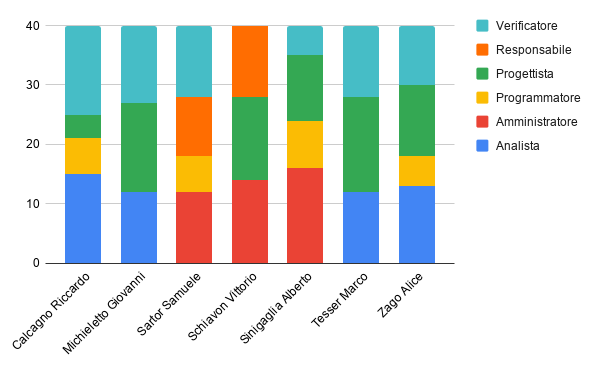
\includegraphics[width=0.8\linewidth]{./res/images/OreProgettazioneArchitetturale.png}
	\caption{Istogramma ore progettazione architetturale.}
	\label{fig: Istogramma ore progettazione architetturale.}
\end{figure}

\subsubsection{Prospetto economico}

In questa fase il costo per ogni ruolo è il seguente:
\begin{longtable}{|c|c|c|}
	\hline
	\rowcolor[HTML]{F9CB9C} 
	\textbf{Ruolo} & \textbf{Ore} & \textbf{Costo} \\
	\hline
	Analista &
	52 &
	1300 \\
	\hline
	Amministratore  &
	42 &
	840 \\
	\hline
	Programmatore &
	25 &
	375 \\
	\hline
	Progettista &
	72 &
	1584 \\
	\hline
	Responsabile &
	22 &
	660 \\
	\hline
	Verificatore &
	67 &
	1005 \\
	\hline
	\rowcolor[HTML]{F9CB9C} 
	\textbf{Totale} & \textbf{280} & \textbf{5764} \\
	\hline
	\caption{Costi progettazione architetturale.}
	\label{fig: Costi progettazione architetturale.}
\end{longtable}

I dati ottenuti si possono riassumere nel seguente diagramma circolare:
\begin{figure}[H]
	\centering
	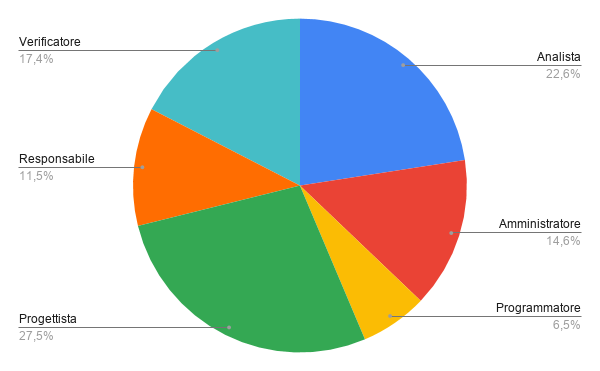
\includegraphics[width=0.6\linewidth]{./res/images/CostiProgettazioneArchitetturale.png}
	\caption{Diagramma circolare costi progettazione architetturale.}
	\label{fig: Diagramma circolare costi progettazione architetturale.}
\end{figure}



			
%
%
% Fase di progettazione di dettaglio requisiti obbligatori
%
%
\subsection{Fase di progettazione di dettaglio requisiti obbligatori}

\subsubsection{Prospetto orario}

Nella fase di progettazione di dettaglio dei requisiti obbligatori ogni componente rivestirà i seguenti ruoli:
\begin{longtable}{|c|c|c|c|c|c|c|c|}
	\hline
	\rowcolor[HTML]{F9CB9C} 
	\textbf{Nominativo} & \textbf{An} & \textbf{Amm} & \textbf{Pr} & \textbf{Pt} & \textbf{Re} & \textbf{Ve} & \textbf{Ore totali} \\
	\hline
	Calcagno Riccardo & 
	- & 
	4 & 
	15 & 
	8 & 
	- & 
	8 & 
	35 \\
	\hline
	Michieletto Giovanni & 
	- & 
	4 & 
	13 & 
	8 & 
	- & 
	10 & 
	35 \\
	\hline
	Sartor Samuele &  
	- & 
	- & 
	18 & 
	9 & 
	- & 
	8 & 
	35 \\
	\hline
	Schiavon Vittorio &  
	- & 
	5 & 
	12 & 
	6 & 
	- & 
	12 & 
	35 \\
	\hline
	Sinigaglia Alberto &  
	- & 
	3 & 
	18 & 
	7 & 
	- & 
	7 & 
	35 \\
	\hline
	Tesser Marco  & 
	- & 
	4 & 
	13 & 
	7 & 
	11 & 
	- & 
	35 \\
	\hline
	Zago Alice & 
	- & 
	- & 
	14 & 
	10 & 
	- & 
	11 & 
	35 \\
	\hline	
	\rowcolor[HTML]{F9CB9C} 
	\textbf{Ore totali ruolo} & \textbf{-} & \textbf{20} & \textbf{103} & \textbf{55} & \textbf{11} & \textbf{56} & \textbf{245} \\
	\hline
	\caption{Prospetto orario progettazione di dettaglio requisiti obbligatori.}
	\label{fig: Prospetto orario progettazione di dettaglio requisiti obbligatori.}
\end{longtable}

I dati ottenuti si possono riassumere nel seguente istogramma:
\begin{figure}[H]
	\centering
	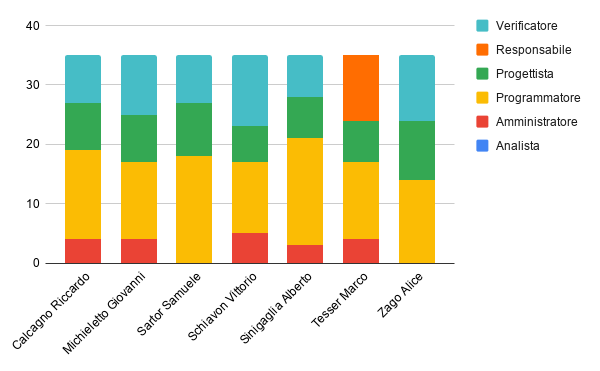
\includegraphics[width=0.8\linewidth]{./res/images/OreObbligatori.png}
	\caption{Istogramma ore progettazione di dettaglio requisiti obbligatori.}
	\label{fig: Istogramma ore progettazione di dettaglio requisiti obbligatori.}
\end{figure}

\subsubsection{Prospetto economico}

In questa fase il costo per ogni ruolo è il seguente:
\begin{longtable}{|c|c|c|}
	\hline
	\rowcolor[HTML]{F9CB9C} 
	\textbf{Ruolo} & \textbf{Ore} & \textbf{Costo} \\
	\hline
	Analista & 
	0 & 
	0 \\
	\hline
	Amministratore &
	20 &
	400 \\
	\hline
	Programmatore &
	103 &
	1545 \\
	\hline
	Progettista &
	55 &
	1210 \\
	\hline
	Responsabile & 
	11 &
	330 \\
	\hline
	Verificatore &
	56 &
	840 \\
	\hline
	\rowcolor[HTML]{F9CB9C} 
	\textbf{Totale} & \textbf{245} & \textbf{4325} \\
	\hline
	\caption{Costi progettazione di dettaglio requisiti obbligatori.}
	\label{fig: Costi progettazione di dettaglio requisiti obbligatori.}
\end{longtable}

I dati ottenuti si possono riassumere nel seguente diagramma circolare:
\begin{figure}[H]
	\centering
	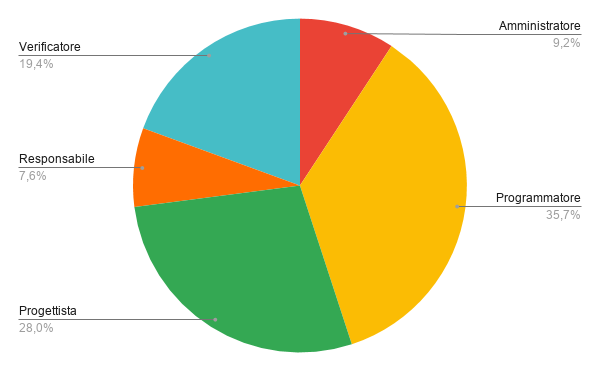
\includegraphics[width=0.6\linewidth]{./res/images/CostiObbligatori.png}
	\caption{Diagramma circolare costi progettazione di dettaglio requisiti obbligatori.}
	\label{fig: Diagramma circolare costi progettazione di dettaglio requisiti obbligatori.}
\end{figure}


%
%
% Fase di progettazione di dettaglio requisiti opzionali 
%
%
\subsection{Fase di progettazione di dettaglio requisiti opzionali }

\subsubsection{Prospetto orario}

Nella fase di progettazione di dettaglio requisiti opzionali ogni componente rivestirà i seguenti ruoli:
\begin{longtable}{|c|c|c|c|c|c|c|c|}
	\hline
	\rowcolor[HTML]{F9CB9C} 
	\textbf{Nominativo} & \textbf{An} & \textbf{Amm} & \textbf{Pr} & \textbf{Pt} & \textbf{Re} & \textbf{Ve} & \textbf{Ore totali} \\
	\hline
	Calcagno Riccardo
	- &
	4 &
	5 &
	2 &
	- &
	4 &
	15 \\
	\hline
	Michieletto Giovanni &
	- &
	- &
	4 &
	- &
	8 &
	3 &
	15 \\
	\hline
	Sartor Samuele & 
	- &
	- &
	5 &
	4 &
	- &
	6 &
	15 \\
	\hline
	Schiavon Vittorio & 
	- &
	2 &
	8 &
	5 &
	- &
	- &
	15 \\
	\hline
	Sinigaglia Alberto & 
	- &
	2 &
	4 &
	4 &
	- &
	5 &
	15 \\
	\hline
	Tesser Marco &
	- &
	- &
	6 &
	6 &
	- &
	3 &
	15 \\
	\hline
	Zago Alice &
	- &
	- &
	9 &
	- &
	- &
	6 &
	15 \\
	\hline	
	\rowcolor[HTML]{F9CB9C} 
	\textbf{Ore totali ruolo} & \textbf{-} & \textbf{8} & \textbf{41} & \textbf{21} & \textbf{8} & \textbf{27} & \textbf{105} \\
	\hline
	\caption{Prospetto orario progettazione di dettaglio requisiti opzionali.}
	\label{fig: Prospetto orario progettazione di dettaglio requisiti opzionali.}
\end{longtable}

I dati ottenuti si possono riassumere nel seguente istogramma:
\begin{figure}[H]
	\centering
	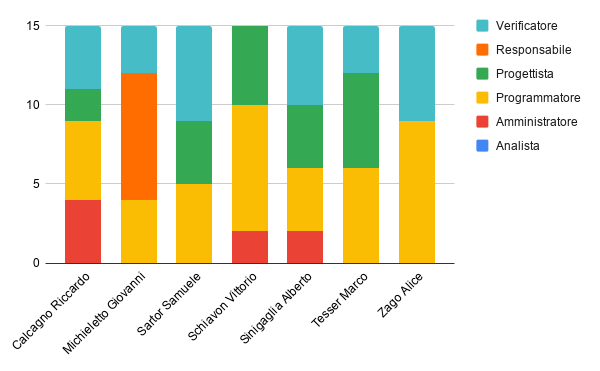
\includegraphics[width=0.8\linewidth]{./res/images/OreOpzionali.png}
	\caption{Istogramma ore progettazione di dettaglio requisiti opzionali.}
	\label{fig: Istogramma ore progettazione di dettaglio requisiti opzionali.}
\end{figure}

\subsubsection{Prospetto economico}

In questa fase il costo per ogni ruolo è il seguente:
\begin{longtable}{|c|c|c|}
	\hline
	\rowcolor[HTML]{F9CB9C} 
	\textbf{Ruolo} & \textbf{Ore} & \textbf{Costo} \\
	\hline
	Analista &
	- &
	-\\
	\hline
	Amministratore &
	8 &
	160 \\
	\hline
	Programmatore &
	41 &
	615 \\
	\hline
	Progettista &
	21 &
	462 \\
	\hline
	Responsabile  &
	8 &
	240 \\
	\hline
	Verificatore &
	27 &
	405 \\
	\hline
	\rowcolor[HTML]{F9CB9C} 
	\textbf{Totale} & \textbf{105} & \textbf{1882} \\
	\hline
	\caption{Costi progettazione di dettaglio requisiti opzionali.}
	\label{fig: Costi progettazione di dettaglio requisiti opzionali.}
\end{longtable}

I dati ottenuti si possono riassumere nel seguente diagramma circolare:
\begin{figure}[H]
	\centering
	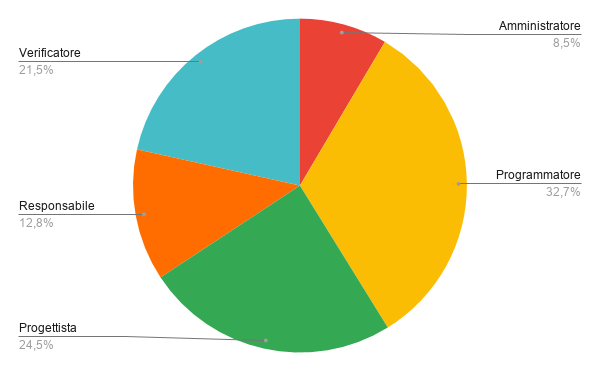
\includegraphics[width=0.6\linewidth]{./res/images/CostiOpzionali.png}
	\caption{Diagramma circolare costi progettazione di dettaglio requisiti opzionali.}
	\label{fig: Diagramma circolare costi progettazione di dettaglio requisiti opzionali.}
\end{figure}			
		
			
%
%
% Fase di 
%
%
\subsection{Fase di validazione e collaudo}

\subsubsection{Prospetto orario}

Nella fase di validazione e collaudo ogni componente rivestirà i seguenti ruoli:
\begin{longtable}{|c|c|c|c|c|c|c|c|}
	\hline
	\rowcolor[HTML]{F9CB9C} 
	\textbf{Nominativo} & \textbf{An} & \textbf{Amm} & \textbf{Pr} & \textbf{Pt} & \textbf{Re} & \textbf{Ve} & \textbf{Ore totali} \\
	\hline
	Calcagno Riccardo &
	- &
	- &
	7 &
	13 &
	- &
	10 &
	30 \\
	\hline
	Michieletto Giovanni &
	- &
	6 &
	11 &
	- &
	- &
	13 &
	30 \\
	\hline
	Sartor Samuele  &
	- &
	8 &
	6 &
	6 &
	- &
	10 &
	30 \\
	\hline
	Schiavon Vittorio  &
	- &
	- &
	13 &
	7 &
	- &
	10 &
	30 \\
	\hline
	Sinigaglia Alberto  &
	- &
	7 &
	10 &
	- &
	7 &
	6 &
	30 \\
	\hline
	Tesser Marco &
	- &
	- &
	12 &
	10 &
	- &
	8 &
	30 \\
	\hline
	Zago Alice &
	- &
	- &
	- &
	9 &
	10 &
	11 &
	30 \\
	\hline	
	\rowcolor[HTML]{F9CB9C} 
	\textbf{Ore totali ruolo} & \textbf{-} & \textbf{21} & \textbf{59} & \textbf{45} & \textbf{17} & \textbf{68} & \textbf{210} \\
	\hline
	\caption{Prospetto orario validazione e collaudo.}
	\label{fig: Prospetto orario validazione e collaudo.}
\end{longtable}

I dati ottenuti si possono riassumere nel seguente istogramma:
\begin{figure}[H]
	\centering
	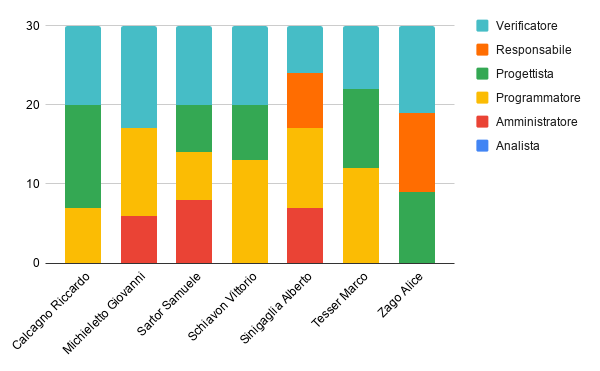
\includegraphics[width=0.8\linewidth]{./res/images/OreValidazioneCollaudo.png}
	\caption{Istogramma ore validazione e collaudo.}
	\label{fig: Istogramma ore validazione e collaudo.}
\end{figure}

\subsubsection{Prospetto economico}

In questa fase il costo per ogni ruolo è il seguente:
\begin{longtable}{|c|c|c|}
	\hline
	\rowcolor[HTML]{F9CB9C} 
	\textbf{Ruolo} & \textbf{Ore} & \textbf{Costo} \\
	\hline
	Analista &
	- &
	- \\
	\hline
	Amministratore &
	21 &
	420 \\
	\hline
	Programmatore &
	59 &
	885 \\
	\hline
	Progettista &
	45 &
	990 \\
	\hline
	Responsabile  &
	17 &
	510 \\
	\hline
	Verificatore &
	68 &
	1020 \\
	\hline
	\rowcolor[HTML]{F9CB9C} 
	\textbf{Totale} & \textbf{210} & \textbf{3825} \\
	\hline
	\caption{Costi validazione e collaudo.}
	\label{fig: Costi validazione e collaudo.}
\end{longtable}

I dati ottenuti si possono riassumere nel seguente diagramma circolare:
\begin{figure}[H]
	\centering
	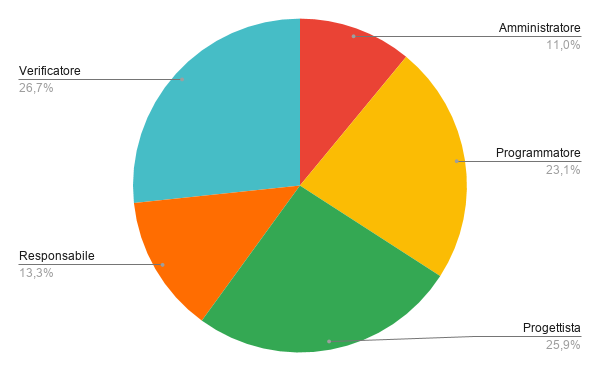
\includegraphics[width=0.6\linewidth]{./res/images/CostiValidazioneCollaudo.png}
	\caption{Diagramma circolare costi validazione e collaudo.}
	\label{fig: Diagramma circolare costi validazione e collaudo.}
\end{figure}
			

%
%
% Riepilogo 
%
%
\subsection{Riepilogo}

\subsubsection{Ore totali non rendicontate}

\paragraph{Prospetto orario non rendicontato}

Viene in seguito riportato il prospetto delle ore di investimento non rendicontate che il team dedicherà ad ogni ruolo:
\begin{longtable}{|c|c|c|c|c|c|c|c|}
	\hline
	\rowcolor[HTML]{F9CB9C} 
	\textbf{Nominativo} & \textbf{An} & \textbf{Amm} & \textbf{Pr} & \textbf{Pt} & \textbf{Re} & \textbf{Ve} & \textbf{Ore totali} \\
	\hline
	Calcagno Riccardo &
	6 &
	5 &
	- &
	- &
	10 &
	15 &
	36 \\
	\hline
	Michieletto Giovanni &
	16 &
	8 &
	- &
	- &
	- &
	12 &
	36 \\
	\hline
	Sartor Samuele &
	10 &
	10 &
	- &
	- &
	- &
	16 &
	36 \\
	\hline
	Schiavon Vittorio & 
	15 &
	- &
	- &
	5 &
	- &
	16 &
	36 \\
	\hline
	Sinigaglia Alberto & 
	15 &
	- &
	- &
	- &
	6 &
	15 &
	36 \\
	\hline
	Tesser Marco &
	20 &
	6 &
	- &
	6 &
	- &
	4 &
	36 \\
	\hline
	Zago Alice &
	12 &
	8 &
	- &
	- &
	- &
	16 &
	36 \\
	\hline	
	\rowcolor[HTML]{F9CB9C} 
	\textbf{Ore totali ruolo} & \textbf{94} & \textbf{37} & \textbf{-} & \textbf{11} & \textbf{16} & \textbf{94} & \textbf{252} \\
	\hline
	\caption{Prospetto orario totale non rendicontato.}
	\label{fig: Prospetto orario totale non rendicontato.}
\end{longtable}

I dati ottenuti si possono riassumere nel seguente istogramma:
\begin{figure}[H]
	\centering
	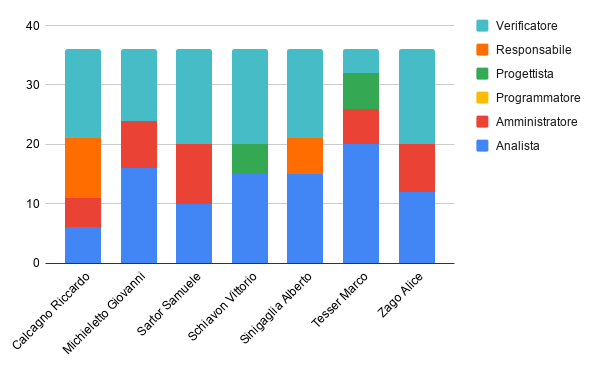
\includegraphics[width=0.8\linewidth]{./res/images/OreNonRendicontate.png}
	\caption{Istogramma ore totali non rendicontate.}
	\label{fig: Istogramma ore totali non rendicontate.}
\end{figure}

\subsubsection{Prospetto economico}

In questa fase il costo per ogni ruolo è il seguente:
\begin{longtable}{|c|c|c|}
	\hline
	\rowcolor[HTML]{F9CB9C} 
	\textbf{Ruolo} & \textbf{Ore} & \textbf{Costo} \\
	\hline
	Analista &
	94 &
	2350 \\
	\hline
	Amministratore &
	37 &
	740 \\
	\hline
	Programmatore &
	- &
	- \\
	\hline
	Progettista &
	11 &
	242 \\
	\hline
	Responsabile &
	16 &
	480 \\
	\hline
	Verificatore &
	94 &
	1410 \\
	\hline
	\rowcolor[HTML]{F9CB9C} 
	\textbf{Totale} & \textbf{252} & \textbf{5222} \\
	\hline
	\caption{Costi totali non rendicontati.}
	\label{fig: Costi totali non rendicontati.}
\end{longtable}

I dati ottenuti si possono riassumere nel seguente diagramma circolare:
\begin{figure}[H]
	\centering
	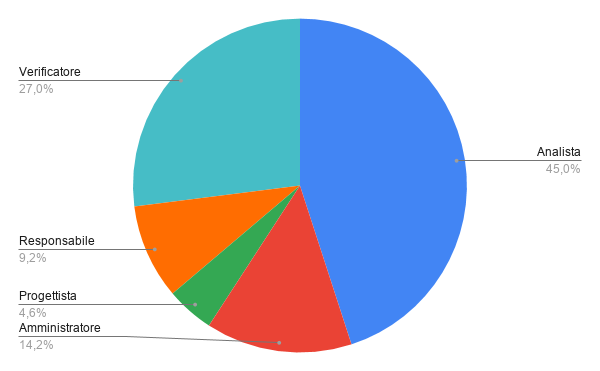
\includegraphics[width=0.6\linewidth]{./res/images/CostiNonRendicontati.png}
	\caption{Diagramma circolare costi totali non rendicontati.}
	\label{fig: Diagramma circolare costi totali non rendicontati.}
\end{figure}

\subsubsection{Ore totali rendicontate}

\paragraph{Prospetto orario rendicontato}

Viene in seguito riportato il prospetto delle ore di investimento, preventivate a carico del committente, che il team dedicherà ad ogni ruolo:
\begin{longtable}{|c|c|c|c|c|c|c|c|}
	\hline
	\rowcolor[HTML]{F9CB9C} 
	\textbf{Nominativo} & \textbf{An} & \textbf{Amm} & \textbf{Pr} & \textbf{Pt} & \textbf{Re} & \textbf{Ve} & \textbf{Ore totali} \\
	\hline
	Calcagno Riccardo &
	15 &
	8 &
	33 &
	27 &
	- &
	37 &
	120 \\
	\hline
	Michieletto Giovanni &
	12 &
	10 &
	28 &
	23 &
	8 &
	39 &
	120 \\
	\hline
	Sartor Samuele & 
	- &
	20 &
	35 &
	19 &
	10 &
	36 &
	120 \\
	\hline
	Schiavon Vittorio & 
	- &
	21 &
	33 &
	32 &
	12 &
	22 &
	120 \\
	\hline
	Sinigaglia Alberto & 
	- &
	28 &
	40 &
	22 &
	7 &
	23 &
	120 \\
	\hline
	Tesser Marco &
	12 &
	4 &
	31 &
	39 &
	11 &
	23 &
	120 \\
	\hline
	Zago Alice &
	13 &
	- &
	28 &
	31 &
	10 &
	38 &
	120 \\
	\hline	
	\rowcolor[HTML]{F9CB9C} 
	\textbf{Ore totali ruolo} & \textbf{52} & \textbf{91} & \textbf{228} & \textbf{193} & \textbf{58} & \textbf{218} & \textbf{840} \\
	\hline
	\caption{Prospetto orario totale rendicontato.}
	\label{fig: Prospetto orario totale rendicontato.}
\end{longtable}

I dati ottenuti si possono riassumere nel seguente istogramma:
\begin{figure}[H]
	\centering
	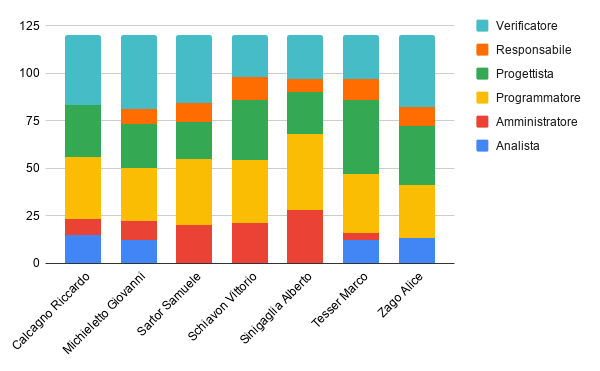
\includegraphics[width=0.8\linewidth]{./res/images/OreRendicontate.png}
	\caption{Istogramma ore totali rendicontate.}
	\label{fig: Istogramma ore totali rendicontate.}
\end{figure}

\subsubsection{Prospetto economico}

In questa fase il costo per ogni ruolo è il seguente:
\begin{longtable}{|c|c|c|}
	\hline
	\rowcolor[HTML]{F9CB9C} 
	\textbf{Ruolo} & \textbf{Ore} & \textbf{Costo} \\
	\hline
	Analista &
	52 &
	1300 \\
	\hline
	Amministratore &
	91 &
	1820 \\
	\hline
	Programmatore &
	228 &
	3420 \\
	\hline
	Progettista &
	193 &
	4246 \\
	\hline
	Responsabile &
	58 &
	1740 \\
	\hline
	Verificatore &
	218 &
	3270 \\
	\hline
	\rowcolor[HTML]{F9CB9C} 
	\textbf{Totale} & \textbf{840} & \textbf{15796} \\
	\hline
	\caption{Costi totali rendicontati.}
	\label{fig: Costi totali rendicontati.}
\end{longtable}

I dati ottenuti si possono riassumere nel seguente diagramma circolare:
\begin{figure}[H]
	\centering
	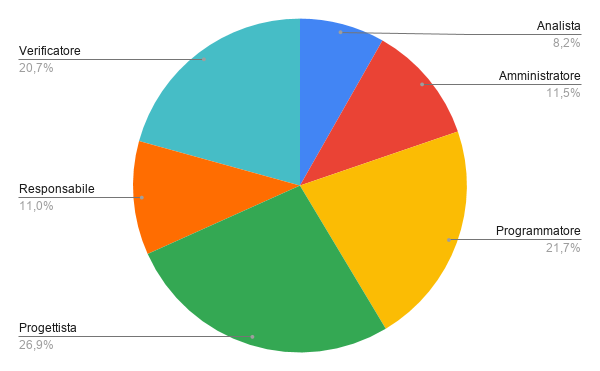
\includegraphics[width=0.6\linewidth]{./res/images/CostiRendicontati.png}
	\caption{Diagramma circolare costi totali rendicontati.}
	\label{fig: Diagramma circolare costi totali rendicontati.}
\end{figure}
			
\subsubsection{Conclusioni}		
Da quanto si può evincere dalle ultime tabelle il costo totale delle ore non rendicontate non è trascurabile. Questo è dovuto al fatto che il team non possiede, almeno inizialmente, le conoscenze e l’esperienza adeguate per svolgere il progetto in modo lineare e quantificare il lavoro di autoformazione in modo preciso. Di conseguenza le ore di autoformazione per ogni ruolo hanno fatto crescere il monte ore totale non rendicontate con il conseguente lievitare dei costi.
\\
Il costo totale preventivato per il progetto sarà quindi €15.796.
